\documentclass[titlepage=firstcover, captions=tableheading]{scrartcl}
\usepackage{microtype}
\usepackage{amsmath}
\usepackage{polyglossia}
\usepackage{graphicx}
\usepackage{booktabs}
\usepackage{siunitx}
\usepackage{hyperref}
\usepackage{caption}
\usepackage{float}
%\usepackage[version=4]{mhchem}
\usepackage{chemformula}
\let\ce\ch
\setdefaultlanguage{german}
\title{V702 Aktivierung mit Neutronen}
\author{
Connor Magnus Böckmann \\ email: \href{mailto:connormagnus.boeckmann@tu-dortmund.de}{connormagnus.boeckmann@tu-dortmund.de}
\and Tim Theissel \\ email: \href{mailto:tim.theissel@tu-dortmund.de}{tim.theissel@tu-dortmund.de}}
\begin{document}
\maketitle
\newpage
\tableofcontents
\newpage
\section{Zielsetzung}
Der folgende Versuch dient der experimentellen Bestimmung der Halbwertszeiten und Zerfallskurven von verschiedenen radioaktiven Isotopen und Isotopengemische mit Hilfe von Neutronenstrahlung.
\section{Theoretische Grundlagen}
Die Stabilitaet, des aus Protonen und Neutronen bestehenden Kerns eines Atoms, haengt von dem Verhaeltnis zwischen Neutronen und Protonen ab. Sollte bei einem Kern das Verhaeltnis ausserhalb des Stabilitaetsbereichs liegen, wandelt sich der Kern mit einer bestimmten Wahrscheinlichkeit in einen stabilen oder in einen instabilen Kern um. Dieser instabile Kern zerfaellt dann weiter. Die Zerfallswahrscheinlichkeit wird durch die Halbwertszeit T ausgedrueckt. Diese Halbwertszeit ist der Zeitraum, in dem von einer grossen Anzahl an Kernen gerade die Haelfte zerfallen ist. Dieses Zeitintervall kann dabei sehr unterschiedliche Laengen annehmen. Die Variation erstreckt sich dabei ueber 23 Zehnerpotenzen. Kernphysikalisch ist T eine bedeutsame Groesse, weshalb es entscheidend ist, diese zu bestimmen. Dafuer gibt es verschiedene Methoden.\\
Die im Folgenden benutzte Methode ermoeglicht eine Bestimmung im Bereich von Sekunden bis Stunden. Um eine akkurate Messung zu ermoeglichen, muessen die Nuklide direkt vor der Messung hergestellt werden, um die Messung nicht zu verfaelschen. Eine einfache und verlaessliche Methode dafuer stellt der Beschuss von stabilen Kernen mit Neutronen dar. Vorteil dieser Methode ist die fehlende elektrische Ladung der Neutronen, weshalb sie nicht die Coulomb-Barriere ueberwinden muessen. \\
Auf die Wechselwirkung von Neutronen mit Kernen, die Erzeugung freier Neutronen, sowie das Messverfahren zur Bestimmung der Halbwertszeit samt geeignetem Messaufbau soll in den folgenden Abschnitten tiefer eingegangen werden.
\subsection{Kernreaktionen mit Neutronen}
Als Kernreaktionen werden alle Wechselwirkungen von Teilchen mit Atomkernen bezeichnet. Speziell die Reaktion von Neutronen mit dem Kern sind hier von Interesse fuer den Versuch. Absorbiert der Ursprungskern A ein Neutron bildet sich ein so genannter Compoundkern A*. Energetisch liegt dieser um die kinetische Energie und die Bindungsenergie des Neutron hoeher als A. Dabei wird die hinzugekommene Energie gleichmaessig auf die Nukleonen verteilt. Dies ruehrt von den starken Wechselwirkungen des neuen Neutron mit dem Kern her. Die Nukleonen werden dadurch in hoehere Energiezustaende versetzt. Es wird von einer so genannten Aufheizung von A* gesprochen. Haeufig ist der Kern dabei nicht in der Lage ein Nukleonen abzustossen, wenn die kinetische Energie des eintreffenden Neutronen nur gering war. Es laeuft eine Reaktion ab, bei der der Kern nach etwa $10^{-16}s$ unter Emission eines \gamma-Quants zurueck in den Grundzustand faellt. Die Reaktion laeuft dabei folgendermassen ab:
\begin{equation}
    \ce{^{m+}_zA + ^{1}_{0}C -> ^{m+1}_zA^{*} -> ^{m+1}_zA + \gamma} \nonumber
\end{equation}
Die Massenzahl wird dabei durch m ausgedrueckt. Der nun entstandene Kern $\ce{^{m+1}_{z}A^{*}}$ ist meistens nicht stabil, da dieser nun mehr Neutronen als ein normaler, stabiler Kern enthaelt. Dieser ist verhaeltnismaessig langlebig im Vergleich mit dem Zwischenkern, auf Grund des Energieverlustes ueber den \gamma-Quant. Der Kern wird nun in einen stabilen Kern umgewandelt. Die Emission eines Elektronen, welche dafuer benoetigt wird, erfolgt folgendermassen:
\begin{equation}
    \ce{^{m+1}_zA -> ^{m+1}_{z+1}C + \beta^- + $E_{kin}$ + $\bar{v\textsubscript{e}}$} \nonumber
\end{equation}
$\bar{v}_e$ stellt dabei ein Antineutrino dar. Die Summe der einzelnen Massen der Teilchen ist dabei geringfuegig kleiner, als die Masse des Kerns $\ce{^{m+1}_zA}$. Der so genannte Massendefekt wird entsprechend der Einsteinschen Beziehung $\Delta E= \Delta mc^{2}$ in kinetische Energie und Antineutrino umgewandelt.\\
Entscheidend fuer die Wahrscheinlichkeit des Einfangens eines Neutrons ist der Wirkungsquerschnitt \sigma. Es ist die Flaeche, welche der Kern haben muesste, damit jedes auftreffende Neutron eingefangen wuerde. Wenn ein ein $1cm^2$-Stueck Folie mit der Dicke d und K Atomen pro $cm^3$ von n Neutronen pro Sekunde getroffen wird, wobei u Einfaenge geschehen, wird \sigma gegeben durch
\begin{equation}
    \sigma =\frac{u}{nKd} \nonumber
\end{equation}
gegeben. Der Wirkungsquerschnitt hat die Einheit $10^{-24}cm^2=:1 barn$. Der Neutroneneinfang und damit der Wirkungsquerschnitt ist stark abhaengig von der Geschwindigkeit der Neutronen. Daher unterscheidet man schnelle und langsame Neutronen mit dem Kriterium der De-Broglie-Wellenlaenge \lambda.  Ein Neutron der Geschwindigkeit v hat eine Wellenlaenge nach De Broglie von
\begin{equation} 
    \lambda=\frac{h}{m_nv} \nonumber
\end{equation}
mit dem plankschen Wirkungsquantum h und der Neutronenmasse $m_n$. Ist v so gross, dass die Wellenlaenge verglichen mit dem Kernradius klein ist ($\approx 10^{-12}cm$), lassen sich geometrische Ueberlegungen nutzen, um die Wechselwirkungen des Kerns mit den Neutronen zu beschreiben. Analog geometrisch dazu laesst sich in der Optik Lichtstreuung an einem Objekt beschreiben, welches gross verglichen mit der Wellenlaenge ist. Diese Ueberlegungen sind bei langsamen Neutronen aber nutzlos auf Grund von Interferenzeffekten. Der Wirkungsquerschnitt kann um mehrere Zehnerpotenzen groesser sein als der geometrische Querschnitt. Resonanzabsorption tritt auf, wenn ein Neutron genau die Energie hat wie die Differenz zweier Energieniveaus des Compoundkerns. Dieser kann etwa als ein System harmonischer Oszillatoren mit diskreten Energieeigenwerten aufgefasst werden. Der Wirkungsquerschnitt kann als Funktion der Neutronenenergie beschrieben werden:
\begin{equation}
    \sigma=\sigma_0\sqrt{\frac{E_{r_{i}}}{E}}\frac{\tilde{c}}{(E-E_{r_{i}})^2+\tilde{c}} \nonumber
\end{equation}
$\tilde{c}$ und $c_0$ sind die charakteristischen Konstanten der Kernreaktion. $E_{r_{i}}$ sind die unterschiedlichen Energieniveaus des Compoundkerns. \sigma(E) hat immer dann ein Maximum , wenn die Energie, die einfaellt, gleich der Hoehe eines der Energieniveaus ist. Fuer den Fall, dass $E<<E_r$ ist, laesst sich $(E-E_r)^2$ als quasi konstant annehmen. Daraus folgt:
\begin{equation}
    \sigma\approx\frac{1}{\sqrt{E}}\approx\frac{1}{v} \nonumber
\end{equation}
Der Einfangquerschnitt ist also umgekehrt proportional zur Neutronengeschwindigkeit. Das heisst, dass die Wahrscheinlichkeit fuer das Einfangen steigt je langsamer die Neutronen sind.
\subsection{Erzeugung niederenergetischer Neutronen}
Es werden also niederenergetische Neutronen benoetigt. Im Folgenden soll erklaert werden, wie diese erreicht werden.\\
Die Neutronen werden in diesem Versuch durch Kernreaktionen erzeugt, da Neutronen in der Natur nicht als freies Teilchen vorkommen. Hier werden die Neutronen beim Beschuss von $\ce{^{9}Be}$ mit \alpha-Teilchen freigesetzt.
\begin{equation}
    \ce{^{9}_4Be + ^{4}_{2}$\alpha$ -> ^{12}_{6}C + ^{1}_{0}n} \nonumber
\end{equation}
Die noetigen \alpha-Teilchen stammen aus dem Zerfall von $ \ce{^{226}Ra}$-Kernen. Sie haben ein kontinuierliches Energiespektrum bis zu 13,7 MeV. Abgebremst werden sie durch das Diffundieren durch dickere Materialschichten aus Atomen mit leichten Kernen. Durch elastische Stoesse wird dabei Energie an die leichten Kerne abgegeben. Je aehnlicher die Massen der stossenden Massen, desto besser ist der Bremseffekt. Dadurch ergibt sich Wasserstoff als geeignetster Stosspartner fuer die Neutronen. 
\begin{figure}[H]
    \centering
    \includegraphics[width=0.6\textwidth]{"Quelle_Neutronen.png"}
    \caption{Querschnitt durch die verwendete Quelle fuer Neutronen\\Aus: Anleitung V702 Seite 213}
    \label{Fig:Quelle}
\end{figure}
\noindent Aus diesem Grund wird die Neutronenquelle mit einem Mantel aus Paraffin umgeben, wie in \ref{Fig:Quelle} zu sehen ist. Durch die Stoesse mit den Kernen des Paraffins werden die Neutronen schliesslich auf eine Ernergie gebracht, die den Molekuelen ihrer Umgebung entspricht. Dies entspricht etwa 0,025 eV bei 290 K. Die Neutronengeschwindigkeit entspricht dabei 2,2 km/s. Diese Neutronen nennen sich thermische Neutronen.
\subsection{Untersuchung des Zerfalls instabiler Isotope}
Durch Neutronenstrahlung koennen folgende stabile Isotope in instabile verwandelt werden:
\begin{equation}
    \ce{^{51}Be, ^{55}Mn, ^{79}Br, ^{115}In, ^{127}J, ^{164}Dy, ^{107}Ag, ^{109}Ag, ^{103}Rh} \nonumber
\end{equation}
Um diesen Prozess durchzufuehren, werden Proben dieser Isotope in die Schaechte der Neutronenquelle (\ref{Fig:Quelle}) gesteckt. Durch $\beta^-$-Zerfall werden die erzeugten instabilen Isotope wieder zu stabilen Isotopen. Die Halbwertszeiten erstrecken sich dabei von Sekunden bis Stunden. Die Prozesse laufen folgendermassen ab:
\begin{align}
    \ce{^{51}_{23}V &+ n -> ^{52}_{23}V -> ^{52}_{24}Cr + $\beta^-$ + $\bar{v}_e$} \nonumber \\
    \ce{^{55}_{25}Mn &+ n -> ^{56}_{25}Mn -> ^{56}_{26}Fe + $\beta^-$ + $\bar{v}_e$} \nonumber\\
    \ce{^{79}_{35}Br &+ n -> ^{80}_{35}Br -> ^{80}_{36}Kr + $\beta^-$ + $\bar{v}_e$} \nonumber\\
    \ce{^{115}_{49}In &+ n -> ^{116}_{49}In -> ^{116}_{50}Sn + $\beta^-$ + $\bar{v}_e$} \nonumber\\
    \ce{^{127}_{53}J &+ n -> ^{128}_{53}J -> ^{128}_{54}Xe + $\beta^-$ + $\bar{v}_e$} \nonumber\\
    \ce{^{164}_{66}Dy &+ n -> ^{165}_{66}Dy -> ^{165}_{67}Ho + $\beta^-$ + $\bar{v}_e$} \nonumber\\ 
    \ce{^{107}_{47}Ag &+ n -> ^{108}_{47}Ag -> ^{108}_{48}Cd + $\beta^-$ + $\bar{v}_e$} \nonumber\\
    \ce{^{109}_{47}Ag &+ n -> ^{110}_{47}Ag -> ^{110}_{48}Cd + $\beta^-$ + $\bar{v}_e$} \nonumber\\
\end{align}
\begin{equation}
    \ce{^{103}_{45}Rh + n ->} \begin{cases}\ce{^{104i}_{45}Rh -> ^{104}_{45}Rh + \gamma -> ^{104}_{46}Pd + \beta^{-} + $\bar{v}_e$ \nonumber \\ ^{104}_{45}Rh -> ^{104}_{46}Pd + \beta^{-} + $\bar{v}_e$} \nonumber\end{cases}
\end{equation}
Aufgabe des hier durchzufuehrenden Experiments soll sein, die Halbwertszeiten der obigen Isotope zu bestimmen. Dazu muss der radioaktive Zerfall und seine Gesetzmaessigkeiten bekannt sein.\\
Die Zahl N(t) der nicht zerfallenen Kerne zum Zeitpunkt t gegeben wird durch:
\begin{equation}
    N(t)=N_0e^{-\lambda t} \label{4}
\end{equation}
Die Zahl $N_0$ gibt die zum Zeitpunkt $t=0$ nicht zerfallenen Kerne an. \lambda ist die so genannte Zerfallskonstante. Sie stellt ein Mass fuer die Wahrscheinlichkeit eines Zerfalls vor und ist daher aeusserst wichtig, da sie somit in direktem Zusammenhang mit der Halbwertszeit T steht. 
\begin{equation}
    \frac{1}{2}N_0=N_0e^{-\lambda T}\nonumber
\end{equation}
Daraus folgt schliesslich:
\begin{equation}
    T=\frac{\ln(2)}{\lambda} \nonumber
\end{equation}
Der hier verwendete Weg zur ermittelnden Halbwertszeiten geht ueber die Messung der pro festem Zeitintervall \Delta t  zerfallenen Kerne $N_{\Delta t}(t)$ in Abhaengigkeit von der Zeit. $N_{\Delta t}(t)$ haengt dabei von der Zeit in exponentieller Beziehung ab. Der Definition entsprechend ist 
\begin{equation}
    N_{\Delta t}(t) = N(t) - N(t+\Delta t)
\end{equation}
Es folgt also aus \ref{4} fuer $N_{\Delta t}(t)$:
\begin{align}
    N_{\Delta t}(t)&=N_0e^{-\lambda t}-N_0e^{-\lambda(t+\Delta t)}=N_0(1-e^{-\lambda\Delta t})e^{-\lambda t} \nonumber \\
    \ln(N_{\Delta t}(t))&=\ln N_0(1-e^{-\lambda\Delta t})-\lambda t \nonumber
\end{align}
Dies ist nun ueber eine Ausgleichsgerade bestimmbar, da $\ln(N_0(1-e^{-\lambda\Delta t}))$ konstant ist. Schwierigkeit ist dabei ein geeignetes $\Delta t$ zu waehlen, da zu kleine $\Delta t$ zu statistischen Fehlern und zu grosse $\Delta t$ zu systematischen Fehlern fuehren.
\subsubsection{Rhodium}
Rhodium kommt nach der Aktivierung sowohl in der Form von \ce{^{104}Rh} (90\%), sowie \ce{^{104i}Rh} (10\%) vor. Zweiteres geht nach der Emission eines \gamma-Quants ebenfalls in ersteres Isotop ueber. Auch hier besteht also das Problem, dass zwei verschiedene Prozesse zur gleichen Zeit ablaufen. Um diese zu trennen wird nun die \gamma-Strahlung detektiert und somit kann in die beiden verschiedenen Zerfaelle aufgetrennt werden. Nun kann in langlebige und kurzlebige Isotope unterschieden werden.
\section{Durchfuehrung}
\subsection{Messapparatur}
\begin{figure}[H]
    \centering
    \includegraphics[width=0.6\textwidth]{"Apparatur_Aktivierung.png"}
    \caption{Schematischer Aufbau der Messapparatur\\Aus: Anleitung V702 Seite 217}
    \label{Fig:Apparatur}
\end{figure}
Die oben beschriebenen Messungen werden mit der Apparatur in \ref{Fig:Apparatur} durchgefuehrt. Ein Geiger-Mueller-Zaehlrohr wird genutzt, um einen konstanten Teil der ausgestrahlten \beta- und \gamma-Strahlung zu detektieren. Eine Abschirmung aus Blei soll dabei den Nulleffekt reduzieren. Die Impulse werden verstaerkt und abwechselnd an die Zaehler 1 und 2 geleitet und dort gezaehlt. der Zeitgeber uebernimmt dabei den Wechsel zwischen den Zaehlern und definiert so das Zeitintervall $\Delta t$.
\subsection{Nulleffekt}
Natuerliche Radioaktivitaet und Hoehenstrahlung sorgen am Zaehlrohr fuer Ausschlaege, auch wenn sich keine Probe in der Apparatur befindet. Diese Impulse beeintraechtigen die Messung und muessen daher moeglichst genau bestimmt werden. Dazu wird mit einem Messintervall von t=300s sieben mal die Hintergrundstrahlung gemessen. Diese werden dann aus weiteren Messungen herausgerechnet.
\subsection{Bestimmung der Halbwertszeit bei Vanadium}
Als Beispiel fuer einfachen Zerfall dient in diesem Versuch Vanadium, welches in aktivierter Form in das Zaehlrohr gesteckt wird. Als Messintervalle wird $\Delta t$=30s festgelegt.
\subsection{Bestimmung der Halbwertszeit bei Rhodium}
Eine Halbwertszeitbestimmung eines Isotopengemischs wird am Beispiel von Rhodium durchgefuehrt. Die Messung erfolgt wie bei Vanadium, jedoch wird das Messintervall auf $\Delta t$=15s verringert.
\documentclass[titlepage=firstcover, captions=tableheading]{scrartcl}
\usepackage{microtype}
\usepackage{amsmath}
\usepackage{polyglossia}
\usepackage{graphicx}
\usepackage{booktabs}
\usepackage{siunitx}
\usepackage{hyperref}
\usepackage{caption}
\usepackage{float}
\setdefaultlanguage{german}

\begin{document}
    
\section{Auswertung}

\subsection{Geometrische Abmessungen}

In der Folgenden Tabelle werden die geometrischen Abmessungen der verwendeten Kupferproben dargestellt.
Dabei gibt es für die Kupferfolie eine Höhe (H), eine Breite(b) und eine Dicke (d) sowie einen Durchmesser (D) und eine Länge (L) des Kupferdrahtes.

\begin{center}
    \captionof{table}{Geometrische Abmessungen in cm}
    \begin{tabular}{lllll}
        \toprule
        H & b & d & D & L \\
        \midrule 
        0.026 & 0.028 & 0.00043 & 0.000263 & 173 \\
        \bottomrule
    \end{tabular}
\end{center}

\subsection{Widerstand}

Der Widerstand wurde bei der Durchführung des Versuchs direkt mit einem Multimeter gemessen.
Dafür musste lediglich das Messgerät an den Kupferdraht angeschlossen werden und mit den richtigen Einstellungen zeigt es einen Widerstand von 9.7 \Omega \; an.

\subsection{Hall Effekt}

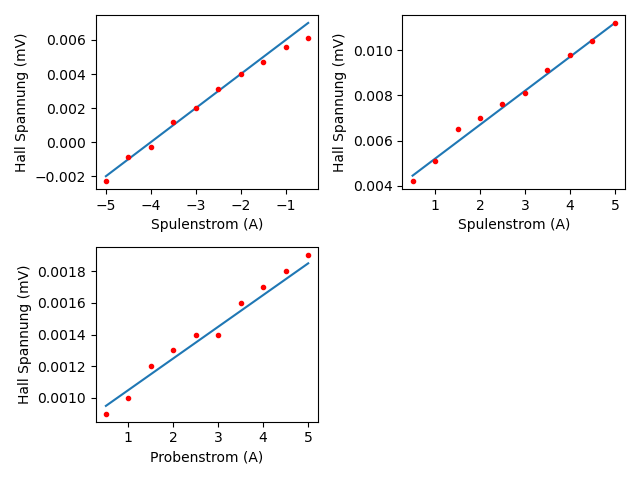
\includegraphics{plothall.png}

In den Koordinatensystemen sind die gemessenen Hall-Spannungen aufgetragen.
Zu den Geaphen ist zu sagen, dass auf der x-Achse entweder der Spulenstrom oder der Probenstrom abgebildet wird.
Die jewils andere Stromstärke wird konstant bei 5A gehalten.

\subsection{Ladungsträger pro Volumen n}

n lässt sich mit der Formel ? brechnen.
Um mit dieser Formel zu rechnen ist es notwendig, die Magnetfeldstärke in abhängigkeit der Stromstärke zu kennen.
Dieser Zusammenhang ist durch die Messwerte gegeben.
Ebenso sind die gemessenen Hall-Spannungen für diese Rechnung notwendig.

Daraus lässt sich die Ladungsdichte bestimmen.

\begin{minipage}{\linewidth}
    \centering
\captionof{table}{Ladungsdichte der Kupferprobe}
\begin{tabular}{ll}
    \toprule
    Stromstärke (A) & Magnetfeldstärke (T) \\
    \midrule
    0.5 &  
    1   &     
    1.5 &  
    2   &  
    2.5 &  
    3   &  
    3.5 &  
    4   &  
    4.5 &  
    5   &      \\
    \bottomrule
    
\end{tabular}
\end{minipage}

\end{document}
\end{document}